\chapter{El teorema de Cauchy-Frobenius-Burnside}

El siguiente resultado se atribuye incorrectamente a Burnside. Se sabe que fue
demostrado independientemente por Cauchy y por Frobenius, para más información
puede consultarse en \cite{MR562002}.
    
\begin{theorem}[Cauchy--Frobenius--Burnside]
    \index{Teorema!de Burnside}
    \index{Burnside!teorema de}
    Supongamos que el grupo $G$ actúa en un conjunto finito $X$. 
    Si $m$ es la cantidad de órbitas de la acción,
    entonces
    \[
    m=\frac{1}{|G|}\sum_{g\in G}|\Fix(g)|,
    \]
    donde $\Fix(g)=\{x\in X:g\cdot x=x\}$.
\end{theorem}
    
\begin{proof}
    Sea $V$ el espacio vectorial con base en $\{x:x\in X\}$. 
    Como $G$ actúa en $X$, 
     tenemos un morfismo
    $\rho\colon G\to\GL(V)$, $g\mapsto\rho_g$. Observemos que para cada $g\in G$ 
    la matriz de $\rho_g$ en la base $\{x:x\in X\}$ es
    \begin{align*}
        (\rho_g)_{ij}=\begin{cases}
            1 & \text{si $g\cdot x_j=x_i$},\\
            0 & \text{en otro caso}.
        \end{cases}
        \shortintertext{En particular,}
        (\rho_g)_{ii}=\begin{cases}
            1 & \text{si $x_i\in\Fix(g)$},\\
            0 & \text{en otro caso}.
        \end{cases}
    \end{align*}
    Si $\chi$ es el caracter de $\rho$, entonces 
    \[
    \chi(g)=\trace(\rho_g)=\sum_{i=1}^k(\rho_g)_{ii}=|\Fix(g)|.
    \]
    Vimos en el lema~\ref{lem:invariantes} que
    $\langle\chi,\chi_1\rangle =\dim V^G$, 
    donde $\chi_1$ denota al caracter trivial. 
    
    Para demostrar el teorema tenemos necesitamos $\dim V^G=m$. 
    
    Sean $x_1,\dots,x_m$ los representantes de las órbitas de la acción de $G$ en $X$. Para cada $i\in\{1,\dots,m\}$ sea
    $v_i=\sum_{x\in G\cdot x_i}x$. Veamos que $\{v_1,\dots,v_m\}$ es una base de $V$. 
    
    Primero vemos que 
    $\{v_1,\dots,v_m\}\subseteq V^G$, pues 
    para cada $g\in G$, tenemos
    \[
    g\cdot v_i=\sum_{x\in G\cdot x_i}g\cdot x=\sum_{y\in G\cdot y}y=v_i,
    \]
    ya que si $x$ recorre una órbita, también lo hace $g\cdot x$. 
    
    El conjunto $\{v_1,\dots,v_m\}$ es linealmente independiente, 
    pues los $v_1,\dots,v_m$ son ortogonales no nulos. De hecho,
    \[
    \langle v_i,v_j\rangle=\begin{cases}
    |G\cdot x_i| & \text{si $i=j$},\\
    0 & \text{en otro caso}.
    \end{cases}
    \]
    
    Veamos que $V$ está generado por el conjunto 
    $\{v_1,\dots,v_m\}$. Si $v\in V^G$, escribimos $v=\sum_{x\in X}\lambda_xx$ 
    para $\lambda_x\in\C$. Afirmamos que si existe $g\in G$ tal que $g\cdot y=z$, entonces
    $\lambda_y=\lambda_z$. En efecto, como $v\in V^G$, tenemos 
    \[
    \sum_{x\in X}\lambda_xx = v = g\cdot v= \sum_{x\in X}\lambda_x(g\cdot x), 
    \]
    de donde obtenemos $\lambda_z=\lambda_y$ 
    al comparar el coeficiente de $z$ en ambos miembros de la igualdad. 
    Podemos escribir 
    entonces 
    \[
    v=\sum_{x\in X}\lambda_xx
    =\sum_{i=1}^m\lambda_{x_i}\sum_{y\in G\cdot x_i}y
    =\sum_{i=1}^m(\lambda_{x_i}|G\cdot x_i|)v_i.\qedhere
    \]
    % \begin{align*}
    % \langle\chi,\chi_1\rangle &=\dim V^G.
    % \end{align*}
\end{proof}

En~\cite{MR1997347} encontramos una 
demostración alternativa muy sencilla. Hagamos el caso en que $G$ actúa transitivamente en $X$: 
\[
\sum_{g\in G}|\Fix(g)|=\sum_{g\in G}\sum_{\substack{x\in X\\g\cdot x=x}}1=\sum_{x\in X}\sum_{\substack{g\in G\\g\cdot x=x}}1=\sum_{x\in X}|G_x|=|G_x||X|=|G|.
\]

El teorema de Cauchy--Frobenius--Burnside tiene muchas aplicaciones.

\begin{example}
Vamos a calcular de cuántas formas pueden colorearse con dos colores --negro y blanco--
los vértices de un cuadrado. Vamos a contar la cantidad de coloreos salvo simetrías. 
Eso significa, por ejemplo, 
que los coloreos 
\begin{equation}
\label{eq:orbita}
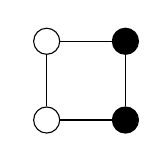
\begin{tikzpicture}
    \node[shape=circle,draw=black,fill=black] (A) at (1,0){};
    \node[shape=circle,draw=black,fill=black] (B) at (1,1){};
    \node[shape=circle,draw=black] (C) at (0,1){}; 
    \node[shape=circle,draw=black] (D) at (0,0){};
    \path [-](A) edge node[left]{} (B);
    \path [-](B) edge node[left]{} (C);
    \path [-](C) edge node[left]{} (D);
    \path [-](D) edge node[left]{} (A);
\end{tikzpicture}
\qquad
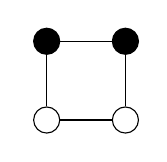
\begin{tikzpicture}
    \node[shape=circle,draw=black] (A) at (1,0) {};
    \node[shape=circle,draw=black,fill=black] (B) at (1,1) {};
    \node[shape=circle,draw=black,fill=black] (C) at (0,1) {};
    \node[shape=circle,draw=black] (D) at (0,0) {};
    \path [-](A) edge node[left]{} (B);
    \path [-](B) edge node[left]{} (C);
    \path [-](C) edge node[left]{} (D);
    \path [-](D) edge node[left]{} (A);
\end{tikzpicture}
\qquad
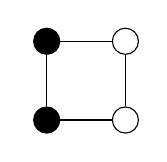
\begin{tikzpicture}
    \node[shape=circle,draw=black] (A) at (1,0) {};
    \node[shape=circle,draw=black] (B) at (1,1) {};
    \node[shape=circle,draw=black,fill=black] (C) at (0,1) {};
    \node[shape=circle,draw=black,fill=black] (D) at (0,0) {};
    \path [-](A) edge node[left]{} (B);
    \path [-](B) edge node[left]{} (C);
    \path [-](C) edge node[left]{} (D);
    \path [-](D) edge node[left]{} (A);
\end{tikzpicture}
\qquad
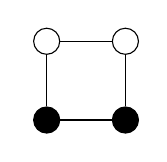
\begin{tikzpicture}
    \node[shape=circle,draw=black,fill=black] (A) at (1,0) {};
    \node[shape=circle,draw=black] (B) at (1,1) {};
    \node[shape=circle,draw=black] (C) at (0,1) {};
    \node[shape=circle,draw=black,fill=black] (D) at (0,0) {};
    \path [-](A) edge node[left]{} (B);
    \path [-](B) edge node[left]{} (C);
    \path [-](C) edge node[left]{} (D);
    \path [-](D) edge node[left]{} (A);
\end{tikzpicture}
\end{equation}
serán considerados equivalentes. Sea $G=\langle g\rangle$ el grupo cíclico de orden cuatro y sea $X$ 
el conjunto de coloreos del cuadrado. 

Obviamente $|X|=16$. 

Hacemos actuar a $G$ en $X$ por 
rotaciones de 90\textdegree~en sentido antihorario. Los coloreos 
que vimos en~\eqref{eq:orbita} están todos en una misma órbita. 
Otra de las órbitas del conjunto $X$ está formada por
\[
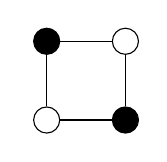
\begin{tikzpicture}
    \node[shape=circle,draw=black,fill=black] (A) at (1,0) {};
    \node[shape=circle,draw=black] (B) at (1,1) {};
    \node[shape=circle,draw=black,fill=black] (C) at (0,1) {};
    \node[shape=circle,draw=black] (D) at (0,0) {};
    \path [-](A) edge node[left]{} (B);
    \path [-](B) edge node[left]{} (C);
    \path [-](C) edge node[left]{} (D);
    \path [-](D) edge node[left]{} (A);
\end{tikzpicture}
\qquad
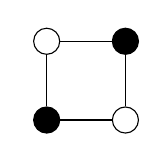
\begin{tikzpicture}
    \node[shape=circle,draw=black] (A) at (1,0) {};
    \node[shape=circle,draw=black,fill=black] (B) at (1,1) {};
    \node[shape=circle,draw=black] (C) at (0,1) {};
    \node[shape=circle,draw=black,fill=black] (D) at (0,0) {};
    \path [-](A) edge node[left]{} (B);
    \path [-](B) edge node[left]{} (C);
    \path [-](C) edge node[left]{} (D);
    \path [-](D) edge node[left]{} (A);
\end{tikzpicture}
\]
La fórmula de Cauchy--Frobenius--Burnside nos dice que
la cantidad de órbitas en $X$ es igual a 
\[
\frac{1}{|G|}\sum_{x\in G}|\Fix(x)|.
\]
Para cada $x\in G=\{1,g,g^2,g^3\}$ calculemos entonces $\Fix(x)$. La identidad fija a los 16 puntos de $X$, 
$g$ y $g^3$ fijan solamente dos puntos de $X$ y 
$g^2$ fija cuatro puntos de $X$. Por ejemplo,
los puntos de $X$ fijados por $g^2$ son
\[
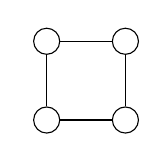
\begin{tikzpicture}
    \node[shape=circle,draw=black] (A) at (1,0){};
    \node[shape=circle,draw=black] (B) at (1,1){};
    \node[shape=circle,draw=black] (C) at (0,1){}; 
    \node[shape=circle,draw=black] (D) at (0,0){};
    \path [-](A) edge node[left]{} (B);
    \path [-](B) edge node[left]{} (C);
    \path [-](C) edge node[left]{} (D);
    \path [-](D) edge node[left]{} (A);
\end{tikzpicture}
\qquad
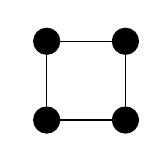
\begin{tikzpicture}
    \node[shape=circle,draw=black,fill=black] (A) at (1,0) {};
    \node[shape=circle,draw=black,fill=black] (B) at (1,1) {};
    \node[shape=circle,draw=black,fill=black] (C) at (0,1) {};
    \node[shape=circle,draw=black,fill=black] (D) at (0,0) {};
    \path [-](A) edge node[left]{} (B);
    \path [-](B) edge node[left]{} (C);
    \path [-](C) edge node[left]{} (D);
    \path [-](D) edge node[left]{} (A);
\end{tikzpicture}
\qquad
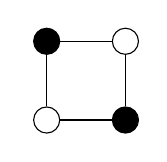
\begin{tikzpicture}
    \node[shape=circle,draw=black,fill=black] (A) at (1,0) {};
    \node[shape=circle,draw=black] (B) at (1,1) {};
    \node[shape=circle,draw=black,fill=black] (C) at (0,1) {};
    \node[shape=circle,draw=black] (D) at (0,0) {};
    \path [-](A) edge node[left]{} (B);
    \path [-](B) edge node[left]{} (C);
    \path [-](C) edge node[left]{} (D);
    \path [-](D) edge node[left]{} (A);
\end{tikzpicture}
\qquad
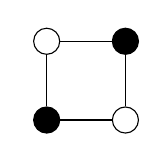
\begin{tikzpicture}
    \node[shape=circle,draw=black] (A) at (1,0) {};
    \node[shape=circle,draw=black,fill=black] (B) at (1,1) {};
    \node[shape=circle,draw=black] (C) at (0,1) {};
    \node[shape=circle,draw=black,fill=black] (D) at (0,0) {};
    \path [-](A) edge node[left]{} (B);
    \path [-](B) edge node[left]{} (C);
    \path [-](C) edge node[left]{} (D);
    \path [-](D) edge node[left]{} (A);
\end{tikzpicture}
\]
Luego $X$ es unión de 
\[
\frac{1}{|G|}\sum_{x\in G}|\Fix(x)|=\frac{1}{4}(16+2+4+2)=6
\]
órbitas. 
\end{example}

\begin{exercise}
Calcule la cantidad de formas (salvo simetrías) en las que pueden ubicarse ocho 
torres en un tablero de ajedrez sin que se ataquen mútuamente. Las simetrías 
de este problema están dadas por la acción del grupo diedral $\D_4$ de ocho elementos. 
\end{exercise}

Si $G$ es un grupo finito, 
se define $\cp(G)$ como la probabilidad de que dos elementos de $G$ 
elegidos al azar conmuten. 
Como aplicación de la fórmula de Cauchy--Frobenius--Burnside 
vamos a demostrar que 
$\cp(G)=k/|G|$, donde $k$ es la cantidad de clases de conjugación de $G$. 

\begin{theorem}[Erd\"os--Turan]
\index{Teorema!5/8}
\index{Teorema!de Erd\"os--Turan}
Si $G$ es un grupo finito no abeliano, entonces $\cp(G)\leq5/8$.
\end{theorem}

\begin{proof}
    Sea $C=\{(x,y)\in G\times G:xy=yx\}$. Veamos que la probabilidad que queremos calcular 
    es
    \[
    \cp(G)=\frac{|C|}{|G|^2}=\frac{k}{|G|}.
    \]
    En efecto, si hacemos actuar a $G$ en $G$ por conjugación. Gracias a 
    la fórmula de Cauchy--Frobenius--Burnside, 
    \[
    k=\frac{1}{|G|}\sum_{g\in G}|\Fix(g)|=\frac{1}{|G|}\sum_{g\in G}|C_G(g)|=\frac{|C|}{|G|},
    \]
    pues $\Fix(g)=\{x\in G:gxg^{-1}=x\}=C_G(g)$ y además $\sum_{g\in G}|C_G(g)|=|C|$. 

    Vamos a demostrar ahora que $k/|G|\leq 5/8$ si $G$ es no abeliano. 
   
    Sean $y_1,\dots,y_m$ representantes de las clases de conjugación de $G$ de tamaño $\geq2$. Por 
    la ecuación de clases, 
    \[
    |G|=|Z(G)|+\sum_{i=1}^m|(G:C_G(y_i))\geq |Z(G)|+2m.
    \]
    Luego $m\leq(1/2)(|G|-|Z(G)|)$ y entonces
    \[
    k=|Z(G)|+m\leq |Z(G)|+\frac12(|G|-|Z(G)|)=\frac12(|Z(G)|+|G|).
    \]
    Como $G$ es no abeliano, el cociente $G/Z(G)$ no es 
    cíclico y entonces, en particular, $(G:Z(G))\geq4$. En consecuencia, 
    \[
    k=\frac12(|Z(G)|+|G|)\leq\frac12\left(\frac14+1\right)|G|,
    \]
    es decir $k/|G|\leq 5/8$. 
\end{proof}

% \begin{example}
%     Sea $G$ un grupo finito con $k$ clases de conjugación. 
%     Como aplicación de la fórmula de Cauchy--Frobenius--Burnside 
%     vamos a demostrar que la probabilidad de que dos elementos elegidos al azar 
%     conmuten es $k/|G|$. 
    
%     Sea $C=\{(x,y)\in G\times G:xy=yx\}$. Veamos que la probabilidad que queremos calcular 
%     es
%     \[
%     \frac{|C|}{|G|^2}=\frac{k}{|G|}.
%     \]
%     Hagamos actuar a $G$ en $G$ por conjugación. Gracias a 
%     la fórmula de Cauchy--Frobenius--Burnside, 
%     \[
%     k=\frac{1}{|G|}\sum_{g\in G}|\Fix(g)|=\frac{1}{|G|}\sum_{g\in G}|C_G(g)|=\frac{|C|}{|G|},
%     \]
%     pues $\Fix(g)=\{x\in G:gxg^{-1}=x\}=C_G(g)$ y además $\sum_{g\in G}|C_G(g)|=|C|$. 
    
%     Vamos a demostrar ahora que $k/|G|\leq 5/8$ si $G$ es no abeliano. 
    
%     Sean $y_1,\dots,y_m$ representantes de las clases de conjugación de $G$ de tamaño $\geq2$. Por 
%     la ecuación de clases, 
%     \[
%     |G|=|Z(G)|+\sum_{i=1}^m|(G:C_G(y_i))\geq |Z(G)|+2m.
%     \]
%     Luego $m\leq(1/2)(|G|-|Z(G)|)$ y entonces
%     \[
%     k=|Z(G)|+m\leq |Z(G)|+\frac12(|G|-|Z(G)|)=\frac12(|Z(G)|+|G|).
%     \]
%     Como $G$ es no abeliano, el cociente $G/Z(G)$ no es 
%     cíclico y entonces, en particular, $(G:Z(G))\geq4$. En consecuencia, 
%     \[
%     k=\frac12(|Z(G)|+|G|)\leq\frac12\left(\frac14+1\right)|G|,
%     \]
%     es decir $k/|G|\leq 5/8$. 
% \end{example}

\begin{exercise}
Demuestre que la probabilidad de que dos elementos elegidos al azar de $Q_8$ 
conmuten es exactamente $5/8$. 
\end{exercise}

\begin{exercise}
Si $G$ es un grupo abeliano y $p$ es el menor primo que divide al orden de $G$, entonces
$\cp(G)\leq (p^2+p-1)/p^3$. Vale además la igualdad si y sólo si $(G:Z(G))=p^2$. 
\end{exercise}

\begin{exercise}
Sea $G$ un grupo finito y sea $H$ un subgrupo de $G$. 
\begin{enumerate}
    \item $\cp(G)\leq\cp(H)$.
    \item Si $H$ es normal en $G$, entonces $\cp(G)\leq\cp(G/H)\cp(H)$.
\end{enumerate}
\end{exercise}

Los grados de las representaciones irreducibles nos dan una cota inferior:

\begin{proposition}
Si $G$ es un grupo finito, entonces
\[
\cp(G)\geq\left(\frac{\sum_{\chi\in\Irr(G)}\chi(1)}{|G|}\right)^2.
\]
\end{proposition}

\begin{proof}
Supongamos que $G$ tiene $k$ clases de conjugación. 
Al usar la desigualdad de Cauchy--Schwarz, 
\begin{align*}
    \left(\sum_{\chi\in\Irr(G)}\chi(1)\right)^2
    &\leq\left(\sum_{\chi\in\Irr(G)}\chi(1)^2\right)\left(\sum_{\chi\in\Irr(G)}1\right)^2
    =\left(\sum_{\chi\in\Irr(G)}\chi(1)^2\right)k=|G|k,
\end{align*}
de donde se obtiene inmediatamente la desigualdad que queríamos demostrar.
\end{proof}

\begin{theorem}[Dixon]
\index{Teorema!de Dixon}
Si $G$ es un grupo finito simple, entonces $\cp(G)\leq1/12$.
% la probabilidad de que dos elementos elegidos al azar 
% conmuten es $\leq1/12$. 
\end{theorem}

El teorema anterior fue propuesto por Dixon como problema en el 
volumen 13 del \emph{Canadian Math. Bulletin} de 1970, 
la solución apareció en 1973. Demostraremos el teorema de Dixon 
cuando estudiemos grupos transitivos.

\begin{exercise}
Verifique que $\cp(\Alt_5)=1/12$. 
\end{exercise}

El grupo alternado $\Alt_5$ juega un papel especial:

\begin{theorem}[Guralnick--Robinson]
\index{Teorema!de Guralnick--Robinson}
Si $G$ es un grupo finito no resoluble y tal que $\cp(G)>3/40$, entonces $G\simeq\Alt_5\times T$ para algún grupo
abeliano $T$ y además $\cp(G)=1/12$. 
\end{theorem}

La demostración puede consultarse en~\cite{MR2228209}.

Veamos otras direcciones hacia donde pueden generalizarse resultados sobre la probabilidad de que dos elementos elegidos al azar conmuten.

En una serie de trabajos monumentales~\cite{MR230809,MR276325,MR313378,MR369512}, 
Thompson demostró el siguiente resultado:

\begin{theorem}[Thompson]
Si $G$ es un grupo finito tal que todo par de elementos de $G$ genera un grupo resoluble, entonces
$G$ es resoluble. 
\end{theorem}

Una demostración mucho más sencilla y que no depende de la clasificación de grupos simples finitos puede consultarse en~\cite{MR1346207}.
El siguiente resultado 
de~\cite{MR1770615} depende de la clasificación de grupos simples, puede 
interpretarse como una versión probabilística del teorema de Thompson.

\begin{theorem}[Guralnick--Wilson]
\index{Teorema!de Guralnick--Wilson}
Sea $G$ un grupo finito. 
\begin{enumerate}
    \item Si la probabilidad de que dos elementos de $G$ elegidos al azar generen un grupo resoluble es $>11/30$, entonces $G$ es resoluble. 
    \item Si la probabilidad de que dos elementos de $G$ elegidos al azar generen un grupo nilpotente es $>1/2$, entonces $G$ es nilpotente.
    \item Si la probabilidad de que dos elementos de $G$ elegidos al azar generen un grupo de orden impar es $>11/30$, entonces $G$ es de orden impar.
\end{enumerate}
\end{theorem}

\index{Orbital}
\index{Rango}
La fórmula de Cauchy--Frobenius--Burnside es útil para determinar caracteres. 

Supongamos que el grupo $G$ actúa en el conjunto finito $X$. Podemos definir entonces
una acción de $G$ en el conjunto $X\times X$:
\[
g\cdot (x,y)=(g\cdot x,g\cdot y).
\]
Las órbitas de esta acción se llaman \textbf{orbitales} de $G$ en $X$. Se define el 
\textbf{rango} de $G$ en $X$ como la cantidad de orbitales de $G$ en $X$. Observemos que
el conjunto de 
puntos fijos de la acción de $g\in G$ en $X\times X$ es 
$\Fix(g)\times\Fix(g)$ pues
\begin{align*}
g\cdot (x,y)=(x,y) &\Longleftrightarrow (g\cdot x,g\cdot y)=(x,y)\\
&\Longleftrightarrow g\cdot x=x,\,g\cdot y=y\Longleftrightarrow (x,y)\in \Fix(g)\times\Fix(g).
\end{align*}
Por el teorema de Cauchy--Frobenius--Burnside, el rango de $G$ en $X$ es igual a 
\[
\frac{1}{|G|}\sum_{g\in G}|\Fix(g)|^2.
\]

\index{Acción!2-transitiva}
Diremos que $G$ actúa \textbf{2-transitivamente} en $X$ si dados $x,y\in X$ con $x\ne y$ 
y $x_1,y_1\in X$ con $x_1\ne y_1$ existe $g\in G$ tal que $g\cdot x=y$ y $g\cdot x_1=y_1$. 

\begin{example}
El grupo simétrico $\Sym_n$ actúa 2-transitivamente en $\{1,2,\dots,n\}$. 
\end{example}

\begin{example}
Si $G$ es 2-transitivo en $X$, entonces el rango de $G$ en $X$ es dos. En efecto, 
un orbital es 
\[
\Delta=\{(x,x):x\in X\}. 
\]
Veamos que el complemento de $\Delta$ es el otro orbital. 
Si $x,y\in X$ y $x_1,y_1\in X$ con $x\ne y$ y $x_1\ne y_1$, 
existe $g\in G$ tal que $g\cdot x=y$ y $g\cdot x_1=y_1$, es decir $g\cdot (x,x_1)=(y,y_1)$. 
\end{example}

\begin{proposition}
Si $G$ actúa 2-transitivamente en $X$ con caracter $\chi$, el caracter 
$\chi-\chi_1$ es irreducible. 
\end{proposition}

\begin{proof}
    Como $G$ actúa 2-transitivamente en $X$, el grupo $G$ es transitivo en $X$. 
    Como el caracter trivial $\chi_1$ es irreducible, $\langle\chi_1,\chi_1\rangle=1$. 
    Por el teorema de Cauchy--Frobenius--Burnside, el rango de $G$ en $X$ es 
    \begin{gather*}
    2=\frac{1}{|G|}\sum_{g\in G}|\Fix(g)|^2=\langle \chi,\chi\rangle.
    \shortintertext{Luego}
    \langle \chi-\chi_1,\chi-\chi_1\rangle=\langle\chi,\chi\rangle-1-1+1=1.\qedhere
    \end{gather*}
\end{proof}

\begin{example}
    El grupo simétrico $\Sym_n$ actúa 2-transitivamente en $\{1,\dots,n\}$. También lo hace el grupo 
    alternado $\Alt_n$ para $n\geq4$. Luego estos grupos poseen un caracter irreducible $\chi$ 
    dado por $\chi(g)=|\Fix(g)|-1$.
\end{example}

\begin{example}
    Sean $p$ un primo y $q=p^{m}$. Sea $V$ el espacio vectorial de dimensión $m$ sobre el cuerpo finito de $q$ elementos. 
    El grupo $G=\GL_2(q)$ actúa 2-transitivamente en el conjunto $X$ de subespacios de $V$ de dimensión uno. En efecto,
    si $\langle v\rangle\ne\langle v_1\rangle$ y $\langle w\rangle\ne\langle w_1\rangle$, 
    entonces $\{v,v_1\}$ y $\{w,w_1\}$ son bases de $V$. 
    La matriz $g$ que corresponde a la transformación lineal $v\mapsto w$, $v_1\mapsto w_1$, es inversible y luego $g\in\GL_2(q)$. 
    La proposición anterior nos da el caracter $\chi(g)=|\Fix(g)|-1$. 
    %Como $V$ tiene $q^2-1$ vectores no nulos
    % y hay $q-1$ subespacios distintos de $V$ que tienen dimensión uno, el caracter
    % $\chi$ que da la proposición anterior tiene grado
    % $\chi(1)=|\Fix(1)|-1=q$. 
\end{example}

Nos basaremos en~\cite{MR1997347} y veremos otras aplicaciones del teorema de Cauchy--Frobenius--Burnside. 

\begin{theorem}[Jordan]
\index{Teorema!de Jordan}
Sea $G$ un grupo finito no trivial. Si $G$ actúa transitivamente en un conjunto finito $X$ y $|X|>1$, entonces
existe $g\in G$ sin puntos fijos. 
\end{theorem}

\begin{proof}
El teorema de Cauchy--Frobenius--Burnside implica que
\[
1=\frac{1}{|G|}\sum_{g\in G}|\Fix(g)|=\frac{1}{|G|}\left(|X|+\sum_{g\ne 1}|\Fix(g)|\right).
\]
Si todo $g\in G\setminus\{1\}$ contiene al menos un punto fijo, entonces
\[
1=\frac{1}{|G|}\left(|X|+\sum_{g\ne 1}|\Fix(g)|\right)\geq \frac{1}{|G|}(|X|+|G|-1)=1+\frac{|X|-1}{|G|}
\]
y luego $|X|\leq1$, una contradicción. 
\end{proof}

\begin{corollary}
Sea $G$ un grupo finito y $H$ un subgrupo propio de $G$. Entonces $G\ne\cup_{g\in G}gHg^{-1}$.
\end{corollary}

\begin{proof}
El grupo $G$ actúa transitivamente en $X=G/H$ por multiplicación a izquierda. 
El estabilizador de $xH$ es 
\[
G_{xH}=\{g\in G:gxH=xH\}=xHx^{-1}.
\]
Como $H\ne G$, entonces $|X|=|G/H|>1$. El teorema de Jordan implica entonces que existe $g\in G$ sin puntos fijos, es decir
que existe $g\in G$ tal que $g\not\in\cup_{x\in G}xHx^{-1}$. 
\end{proof}

Sea $G$ un grupo finito. Diremos que dos clases de conjugación $C$ y $D$ \textbf{conmutan} si existen 
$c\in C$ y $d\in D$ tales que $[c,d]=1$. 
Observemos que $C$ y $D$ conmutan si y sólo si para todo $c\in C$ existe $d\in D$ tal que $[c,d]=1$. 

\begin{corollary}[Wildon]
\index{Teorema!de Wildon}
    Sea $G$ un grupo finito y sea $C$ una clase de conjugación de $G$. Entonces
    $|C|=1$ si y sólo si $C$ conmuta con cualquier clase de conjugación de $G$. 
\end{corollary}
    
\begin{proof}
    Si $C=\{c\}$, entonces $c\in Z(G)$ y luego $C$ conmuta con cualquier clase de conjugación de $G$. Recíprocamente, supongamos que 
    $C$ conmuta con cualquier clase de conjugación de $G$. Si $c\in C$ y $H=C_G(c)$, entonces $H\cap D\ne\emptyset$ para toda
    clase de conjugación $D$. Afirmamos que entonces $G=\cup_{g\in G}gHg^{-1}$. En efecto, sea $x\in G$. Entonces $x\in D$ 
    para alguna clase de conjugación $D$. 
    Sea 
    $h\in H\cap D$. Existe $y\in G$ tal que $h=yxy^{-1}$, es decir $x=y^{-1}hy\in \cup_{g\in G}gHg^{-1}$. Por el teorema de Jordan, 
    $H=G$. Luego $c$ es central, es decir $C=\{c\}$. 
\end{proof}

La clasificación de grupos simples finitos permite demostrar un teorema
similar al teorema de Jordan~\cite{MR636194}. 

\begin{theorem}[Fein--Kantor--Schacher]
\index{Teorema!de Fein--Kantor--Schacher}
Sea $G$ un grupo finito no trivial. Si $G$ actúa transitivamente en un conjunto finito $X$ y $|X|>1$, entonces
existe $g\in G$ de orden una potencia de $p$ sin puntos fijos. 
\end{theorem}

No veremos la demostración en este curso. 

\index{Desarreglos}
Supongamos que $G$ es un grupo finito que actúa fielmente en un conjunto $X$,
digamos $G\leq\Sym_n$, donde $X=\{1,2,\dots,n\}$. Sea 
$G_0$ el conjunto de $g\in G$ sin puntos fijos, es decir $g(x)\ne x$ para todo $x\in X$. 
Tales permutaciones se conocen como \textbf{desarreglos}. 
Sea $c_0=|G_0|/|G|$. 

\begin{theorem}[Cameron--Cohen]
\index{Teorema!de Cameron--Cohen}
Si $G\leq\Sym_n$, entonces $c_0\geq\frac{1}{n}$.
\end{theorem}

\begin{proof}
Sea $X=\{1,\dots,n\}$. El rango de $G$ es, por definición, la cantidad de orbitales de $G$ en $X$. Luego 
el rango de $G$ es $\geq2$, pues $X\times X$ puede descomponerse como 
$X\times X=\Delta\cup\left((X\times X)\setminus\Delta\right)$. 
Sean $\chi(g)=|\Fix(g)|$ y $G_0=\{g\in G:\chi(g)=0\}$. Si $g\not\in G_0$, entonces $1\leq\chi(g)\leq n$. Como 
$(\chi(g)-1)(\chi(g)-n)\leq 0$,
se tiene que 
\[
\frac{1}{|G|}\sum_{g\in G\setminus G_0}(\chi(g)-1)(\chi(g)-n)\leq 0.
\]
Por un lado, 
\begin{align*}
\frac{1}{|G|}\sum_{g\in G}(\chi(g)&-1)(\chi(g)-n)\\
&=\frac{1}{|G|}\left\{\sum_{g\in G_0}+\sum_{g\in G\setminus G_0}\right\}(\chi(g)-1)(\chi(g)-n)\\
&\leq n\frac{|G_0|}{|G|}=nc_0.
\end{align*}
Por otro lado, como el rango de $G$ es $\geq2$, tenemos 
\begin{equation}
    \label{eq:CameronCohen}
    2-\frac{n+1}{|G|}\sum_{g\in G}\chi(g)+n\leq 
    \frac{1}{|G|}\sum_{g\in G}(\chi(g)-1)(\chi(g)-n)\leq nc_0.
\end{equation}
Por hipotesis, $G$ es transitivo en $X$. El teorema de Cauchy--Frobenius--Burnside implica entonces que 
$\sum_{g\in G}\chi(g)=|G|$. Se sigue que $2-(n+1)+n\leq nc_0$ y luego $1/n\leq c_0$. 
% Si $c_0=1/n$, entonces $G$ tiene rango dos (pues si el rango de $G$ es $>2$ entonces la fórmula~\eqref{eq:CameronCohen}
% implica que $1/n<c_0$). Además, por un lado, 
% \begin{align*}
% \frac{1}{|G|}\sum_{g\in G}(\chi(g)-1)(\chi(g)-n)&=\frac{1}{|G|}\sum_{g\in G}\chi(g)^2-\frac{n+1}{|G|}\sum_{g\in G}\chi(g)+n\\
% &=2-(n+1)+n=1.    
% \end{align*}
% Por otro lado, como $c_0=|G_0|/|G|=1/n$, 
% \begin{align*}
% \frac{1}{|G|}\sum_{g\in G}(\chi(g)-1)(\chi(g)-n)
% &=\frac{1}{|G|}\sum_{g\in G\setminus G_0}(\chi(g)-1)(\chi(g)-n)\\
% &=\frac{1}{|G|}\sum_{g\in G_0}(\chi(g)-1)(\chi(g)-n)\\
% &=\frac{1}{|G|}\sum_{g\in G\setminus G_0}(\chi(g)-1)(\chi(g)-n)+1.
% \end{align*}
% Luego $\frac{1}{|G|}\sum_{g\in G\setminus G_0}(\chi(g)-1)(\chi(g)-n)=0$ y entonces $(\chi(g)-1)(\chi(g)-n)$ para todo $g\in G\setminus G_0$.
\end{proof}

El teorema de Cameron--Cohen tiene una segunda parte: 
Si $n$ no es potencia de un primo, entonces $c_0>1/n$. 
Daremos la demostración en el capítulo~\ref{Frobenius}, donde 
estudiaremos grupos de Frobenius.  

La cota del teorema de Cameron--Cohen puede mejorarse si se utiliza la 
clasificación de grupos simples finitos~\cite{MR1484879}.  

\begin{theorem}[Guralnick--Wan]
\index{Teorema!de Guralnick--Wan}
Sea $G$ un grupo finito transitivo de grado $n\geq2$. Si $n$ no es potencia de un 
número primo 
y además $G\ne\Sym_n$ para $n\in\{2,4,5\}$, entonces $c_0\geq 2/n$.
\end{theorem}

La demostración utiliza la clasificación de grupos finitos 2-transitivos, que depende del 
la clasificación de grupos simples finitos.



